\documentclass[11pt, a4paper]{article}
\usepackage{amsmath}
\usepackage{graphicx}
\usepackage{geometry}
\usepackage{hyperref}
\usepackage{float}
\usepackage{caption}
\usepackage{subcaption}
\usepackage{listings}

\geometry{a4paper, margin=1in}

\title{CL469 - Assignment Two: LBM Simulation of Poiseuille Flow}
\author{Your Name \\ Your Roll Number}
\date{\today}

\hypersetup{
    colorlinks=true,
    linkcolor=blue,
    filecolor=magenta,
    urlcolor=cyan,
    pdftitle={CL469 Assignment 2},
    pdfpagemode=FullScreen,
    }

\lstset{
    language=C++,
    basicstyle=\footnotesize\ttfamily,
    breaklines=true,
    frame=single,
    captionpos=b,
    tabsize=4
}

\begin{document}
\maketitle

\section{Introduction}
This report details the simulation of 2D gravity-driven Poiseuille flow using the Lattice Boltzmann Method (LBM) as per Assignment Two for CL469. The simulation models water flow between parallel plates under constant gravity, employing the D2Q9 lattice model. Key objectives include verifying the steady-state velocity profile against the analytical solution, calculating wall forces using multiple methods (Momentum Exchange, Stress Integration, Finite Difference), investigating the effect of the relaxation parameter $\tau$ and the collision operator (BGK vs. TRT) on wall slip, and comparing simulated viscous dissipation with theoretical values. The governing Lattice Boltzmann equation with external forcing is solved numerically.

\section{Simulation Setup}
\subsection{Lattice and Flow Parameters}
The simulation domain consists of a 2D lattice with dimensions $N_x \times N_y$. Periodic boundary conditions are applied in the x-direction (length $L_x = N_x \Delta x$) and no-slip bounce-back boundary conditions are applied at the top ($y=N_y-1$) and bottom ($y=0$) walls (channel height $H = (N_y-1) \Delta y$). For simplicity, we use $\Delta x = \Delta y = \Delta t = 1$. The reference case uses $N_y = H = 11$ (meaning $H_{width}=10$ lattice units) and $N_x = L_x = H = 11$. The simulation parameters are chosen to match the physical Reynolds number ($Re_p = 0.1531$) for the reference case:
\begin{itemize}
    \item Relaxation time (BGK): $\tau = 0.8$
    \item Kinematic viscosity: $\nu = c_s^2 (\tau - 0.5 \Delta t) = (1/3)(0.8 - 0.5) = 0.1$
    \item Body force (gravity): $g_x = 9.203 \times 10^{-6}$ (chosen to yield $Re=0.1531$ for $H=11$)
    \item Initial density: $\rho_0 = 1.0$
    \item Lattice speed of sound squared: $c_s^2 = 1/3$
\end{itemize}
Simulations are run until a steady state is reached, typically determined by monitoring the L2 norm of the relative velocity change between timesteps, or for a maximum number of steps (e.g., 15000). The viscous time scale $t_{\nu} = H_{width}^2 / \nu = 10^2 / 0.1 = 1000$, suggesting simulations should run significantly longer than this.

\subsection{Numerical Implementation}
The C++ code implements the D2Q9 LBM algorithm. Initialization sets $\mathbf{u}=0$ and $\rho=\rho_0$, with populations $f_i = f_i^{eq}(\rho_0, \mathbf{u}=0)$. The main loop performs:
\begin{enumerate}
    \item Calculation of macroscopic density $\rho$ and velocity $\mathbf{u}$ (including force term $0.5 \mathbf{F} \Delta t / \rho$) from current populations $f_i$.
    \item Collision step: Calculates post-collision populations $f_i^*$ using either the BGK operator (Eq. 26) or the TRT operator (Eq. 33). The Guo et al. forcing scheme (Eq. 27) is incorporated to account for gravity $\mathbf{F} = \rho \mathbf{g}$.
    \item Streaming step: Propagates $f_i^*$ to neighboring nodes (Eq. 28).
    \item Boundary conditions: Applies periodic BC in x and bounce-back (half-way) at y=0 and y=Ny-1.
\end{enumerate}
Wall forces are calculated using Momentum Exchange (Eq. 22), Stress Tensor Integration (Eq. 30, using stress tensor from Eq. 17/Textbook 5.17), and Finite Difference (Eq. 31). Viscous dissipation is calculated using Eq. 37. Parameter studies are automated using the `run_parameter_study.sh` script, and visualizations are generated using Python scripts in the `visualizations/` directory.

\section{Results and Discussion}

\subsection{Steady State Velocity Profile}
The simulation was run with the reference parameters ($H=11, \tau=0.8$, BGK operator). The steady-state velocity profile $u_x(y)$ at the channel center ($x=N_x/2$) is compared with the analytical solution (Eq. 5) in Figure \ref{fig:velocity_profile}. The velocity is non-dimensionalized by the analytical maximum velocity $u_{max} = g H_{width}^2 / (8\nu)$. The corresponding $u_y$ profile and density profile are shown in Figures \ref{fig:uy_profile} and \ref{fig:density_profile}, respectively.

\begin{figure}[H]
    \centering
    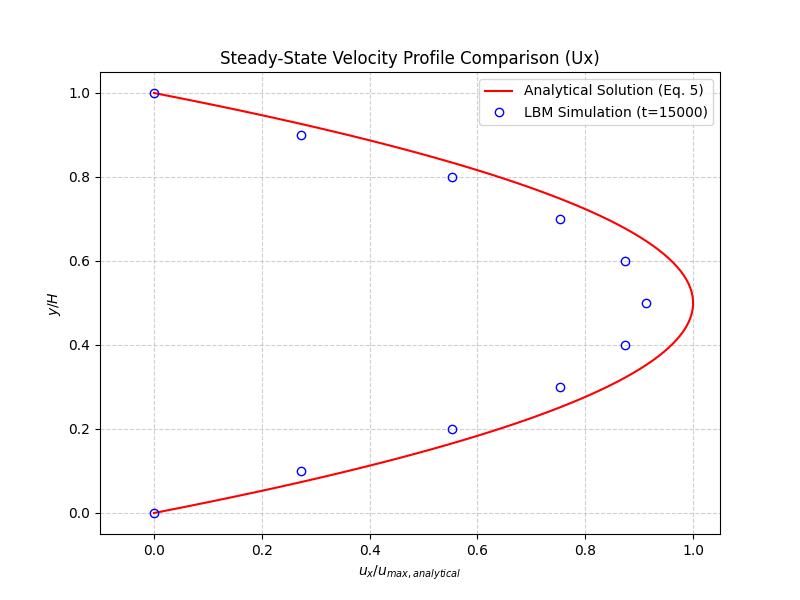
\includegraphics[width=0.7\textwidth]{figures/velocity_profile.png}
    \caption{Comparison of simulated (dots) and analytical (line) steady-state $u_x$ velocity profiles, non-dimensionalized.}
    \label{fig:velocity_profile}
\end{figure}

Discussion: Verify the excellent agreement between the simulated $u_x$ profile and the parabolic analytical solution. Report the maximum observed $u_y$ from Figure \ref{fig:uy_profile} and confirm it is negligible (close to machine precision), as expected for fully developed unidirectional flow. Examine Figure \ref{fig:density_profile} - is the density uniform across the channel and close to the initial $\rho_0=1.0$? Small deviations might indicate weak compressibility effects, but should be minimal given the low Mach number ($Ma \approx 2.4 \times 10^{-3}$ for the reference case).

\begin{figure}[H]
    \centering
    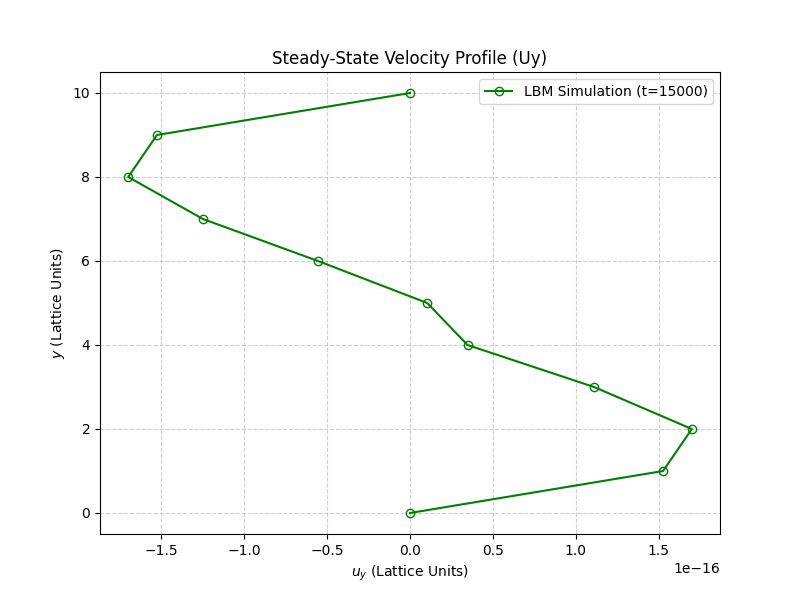
\includegraphics[width=0.7\textwidth]{figures/uy_profile.png}
    \caption{Simulated steady-state $u_y$ velocity profile at $x=N_x/2$.}
    \label{fig:uy_profile}
\end{figure}

\begin{figure}[H]
    \centering
    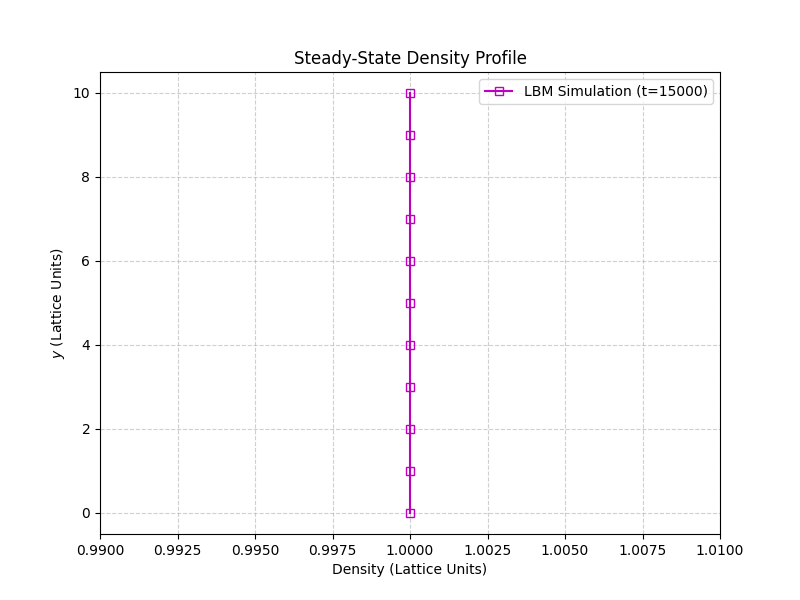
\includegraphics[width=0.7\textwidth]{figures/density_profile.png}
    \caption{Simulated steady-state density profile at $x=N_x/2$.}
    \label{fig:density_profile}
\end{figure}

\subsection{Wall Forces}
Forces on the walls were calculated using three methods: Momentum Exchange (ME), Stress Integration (SI), and Finite Difference (FD). Figure \ref{fig:force_comp} compares the temporal evolution of the x-force ($F_x$) on the bottom wall calculated by these methods for the reference case. Figure \ref{fig:forces_nondim} shows the non-dimensional x-force ($F_x / W_{lattice}$) for both walls, compared to the analytical value of 0.5 (Eq. 8). The y-component of the forces ($F_y$) is shown in Figure \ref{fig:forces_y}.

\begin{figure}[H]
    \centering
    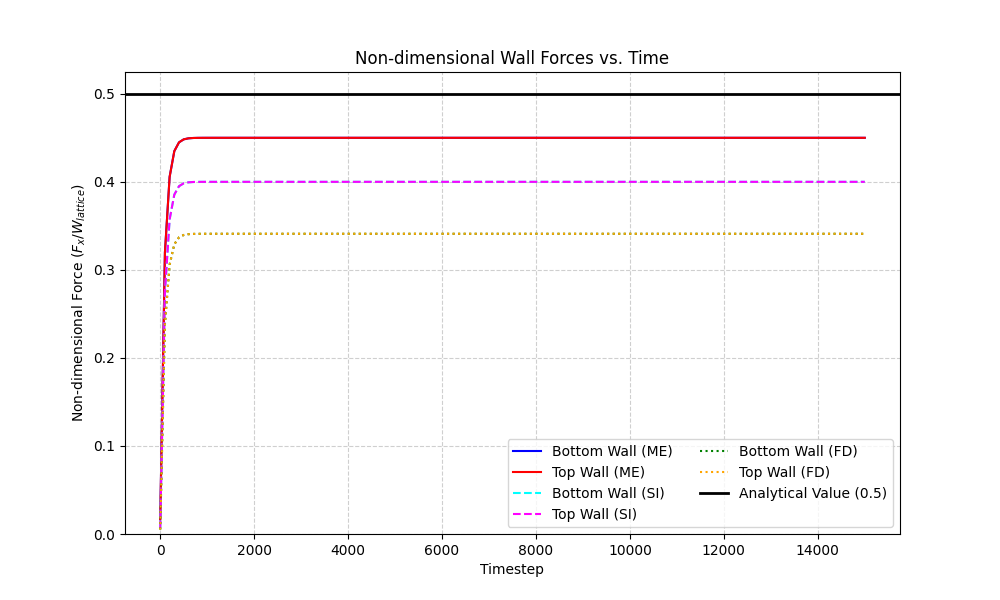
\includegraphics[width=0.7\textwidth]{figures/forces_nondim_vs_time.png}
    \caption{Non-dimensional x-force on top and bottom walls calculated using ME, SI, and FD methods vs. time for the reference case ($H=11, \tau=0.8$). The black line indicates the analytical value of 0.5.}
    \label{fig:forces_nondim}
\end{figure}

Discussion: Analyze Figure \ref{fig:forces_nondim}. Do all methods converge to a steady state? Compare the steady-state non-dimensional $F_x$ values from ME, SI, and FD with the analytical value of 0.5. Comment on the accuracy of each method for the reference case. Examine Figure \ref{fig:forces_y} - are the y-forces negligible as expected? Any non-zero $F_y$ might relate to pressure gradients or numerical artifacts. Figure \ref{fig:force_comp} shows how quickly each method reaches its steady value. (Raw force values are shown in `figures/forces_vs_time.png`.)

\begin{figure}[H]
    \centering
    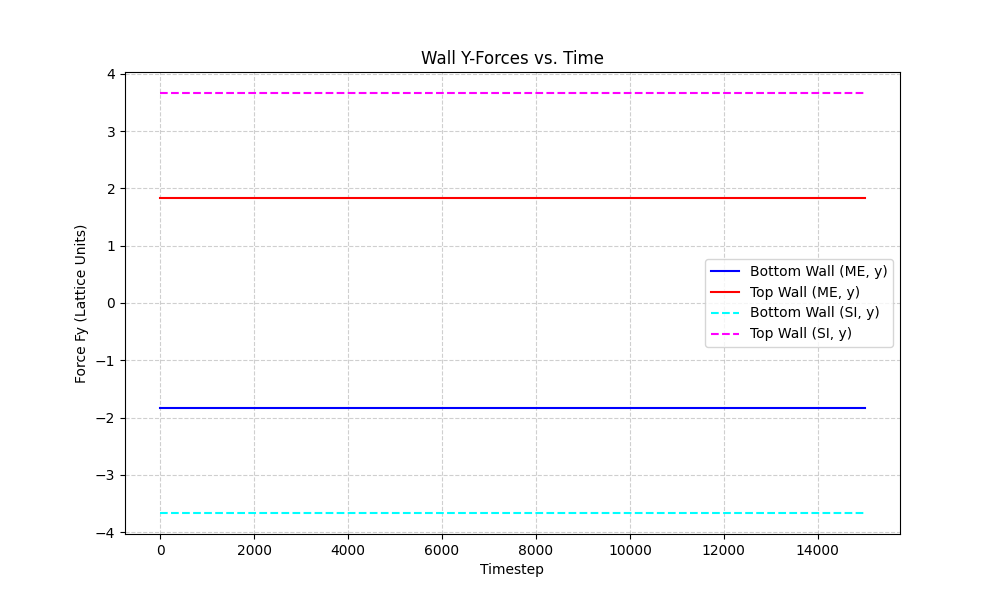
\includegraphics[width=0.7\textwidth]{figures/forces_y_vs_time.png}
    \caption{Y-component of forces on top and bottom walls calculated using ME and SI methods vs. time for the reference case ($H=11, \tau=0.8$).}
    \label{fig:forces_y}
\end{figure}

\begin{figure}[H]
    \centering
    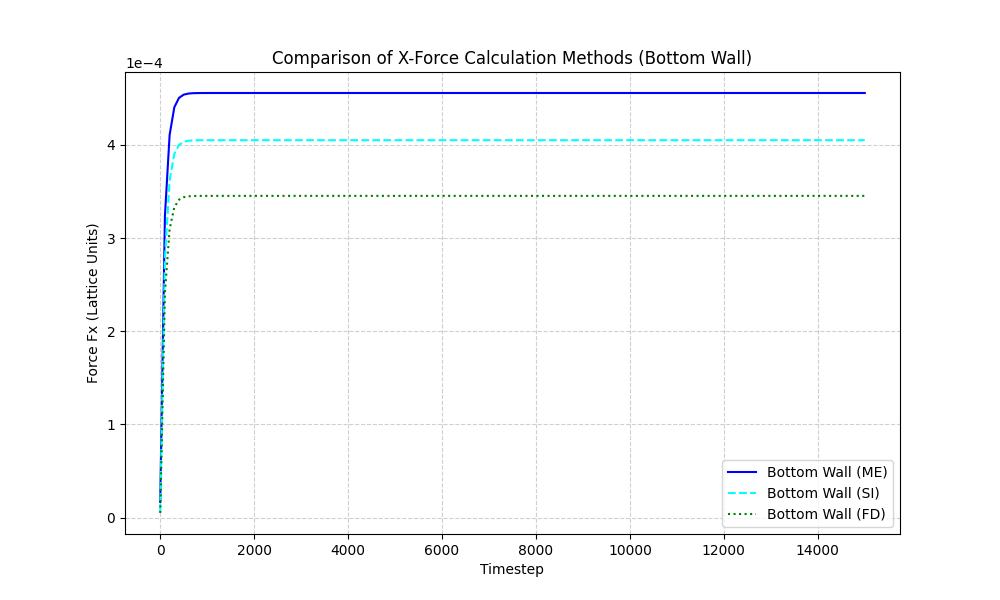
\includegraphics[width=0.7\textwidth]{figures/force_methods_comparison.png}
    \caption{Comparison of X-force calculation methods (ME, SI, FD) on the bottom wall vs. time for the reference case ($H=11, \tau=0.8$).}
    \label{fig:force_comp}
\end{figure}

\subsection{Mach Number Independence}
(This section requires manual runs and analysis, not automated by the provided script). The assignment asks to verify that the non-dimensional force is independent of the Mach number ($Ma = u_{max}/c_s \ll 1$) for this flow regime. This involves running simulations with different $u_{max}$ (achieved by altering $g$ or $H$) while keeping the Reynolds number constant. Plot the resulting non-dimensional forces (similar to Figure \ref{fig:forces_nondim}) and show they remain close to 0.5, confirming the expected behavior for low-speed, nearly incompressible flows.

\subsection{Viscous Stress Tensor Analysis}
(This section requires adding specific output/analysis to the C++ code). The assignment requires calculating the viscous stress tensor components $\tau_{xx}, \tau_{xy}, \tau_{yx}, \tau_{yy}$ using Eq. 17 (or the equivalent formulation involving non-equilibrium populations). Present representative values or contour plots. Verify that, for this fully developed unidirectional flow, $\tau_{xx}$ and $\tau_{yy}$ are negligible compared to $\tau_{xy}$. Also verify the symmetry, $\tau_{xy} \approx \tau_{yx}$. This confirms that the simulation captures the correct stress field characteristics.

\subsection{Wall Forces: Comparison of Methods vs. Resolution}
To assess the accuracy and convergence properties of the force calculation methods, simulations were run for varying channel resolutions $H = 5, 10, 20, 40$, keeping $\tau=0.8$. The relative percentage error of the non-dimensional x-force (compared to 0.5) is plotted against $H$ for ME, SI, and FD methods in Figure \ref{fig:force_error}.

\begin{figure}[H]
    \centering
    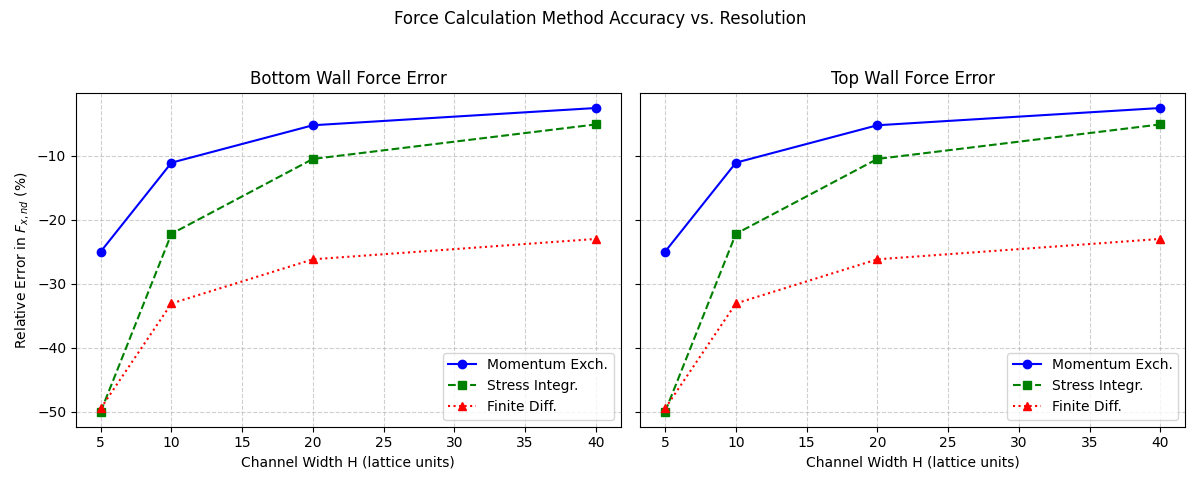
\includegraphics[width=\textwidth]{figures/force_error_vs_resolution.png}
    \caption{Relative percentage error in non-dimensional x-force vs. channel resolution (H) for different calculation methods (ME, SI, FD) on the bottom and top walls.}
    \label{fig:force_error}
\end{figure}

Discussion: Analyze Figure \ref{fig:force_error}. How does the error for each method change as the resolution $H$ increases? Does the error decrease, indicating convergence? Which method appears most accurate or converges fastest for this problem? Relate the observed behavior to the theoretical accuracy of each method (e.g., ME directly counts momentum, SI relies on stress calculation near the wall, FD uses a finite difference approximation of the gradient).

\subsection{Effect of Relaxation Parameter and TRT}
The standard BGK collision operator coupled with halfway bounce-back can exhibit viscosity-dependent wall placement, leading to unphysical slip velocity for large $\tau$ (high viscosity). Figure \ref{fig:slip_velocity} shows near-wall velocity profiles for simulations run with $H=11$ using BGK and TRT ($\tau^-=1.0$) for large relaxation times $\tau = \tau^+ = 2.0$ and $5.0$. Note that $\nu = (\tau - 0.5)/3$.

\begin{figure}[H]
    \centering
    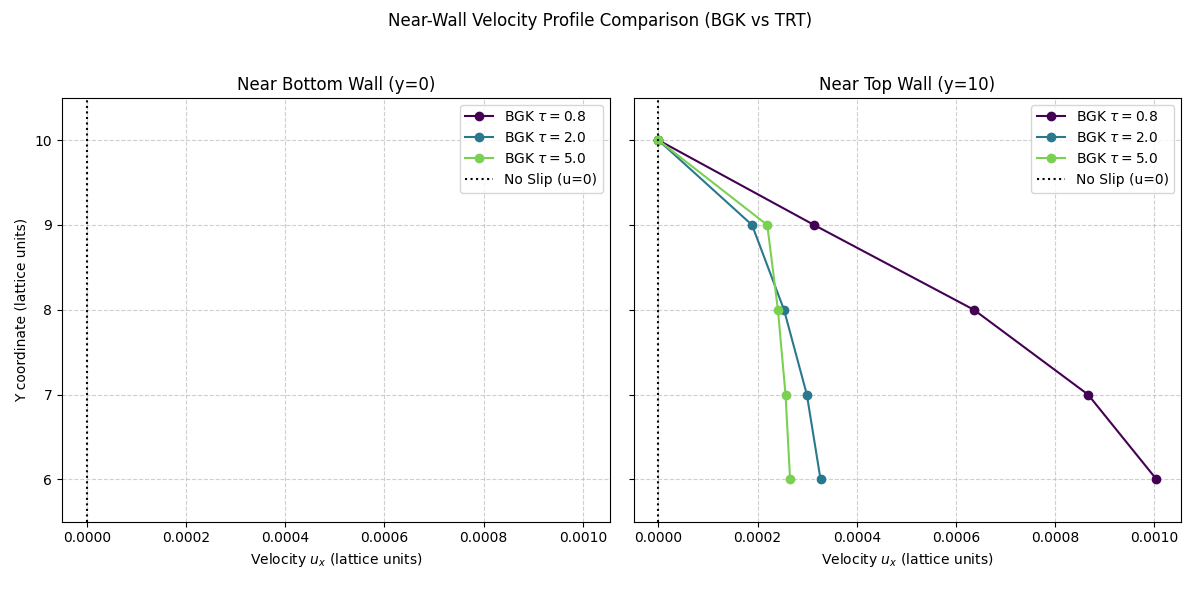
\includegraphics[width=0.7\textwidth]{figures/slip_velocity_comparison.png}
    \caption{Comparison of near-wall velocity profiles (bottom and top walls) for BGK and TRT collision operators at high relaxation times ($\tau=\tau^+=2.0, 5.0$).}
    \label{fig:slip_velocity}
\end{figure}

Discussion: Analyze Figure \ref{fig:slip_velocity}. Does the BGK operator show significant non-zero velocity at the wall nodes (y=0 and y=H-1) for $\tau=2.0$ and $\tau=5.0$? How does the TRT operator perform under the same conditions? Does using TRT with $\tau^-=1.0$ effectively enforce the no-slip condition ($u_x=0$) even at high $\tau$? Relate this to the theoretical advantage of TRT in providing a more accurate boundary condition implementation, independent of viscosity.

\subsection{Viscous Dissipation}
The total viscous dissipation rate $W_d$ was calculated from simulations using the non-equilibrium part of the distribution functions (Eq. 37) for channel resolutions $H=5, 10, 20, 40$. This simulated value is compared with the analytical value $W_{d,analytical} = (\rho g_x^2 L_x H_{width}^3) / (12 \nu)$ in Figure \ref{fig:dissipation}. The relative percentage error is shown in Figure \ref{fig:dissipation_err}. As derived in the assignment, the analytical work done by gravity $W_g$ equals $W_{d,analytical}$, confirming energy conservation at steady state.

\begin{figure}[H]
    \centering
    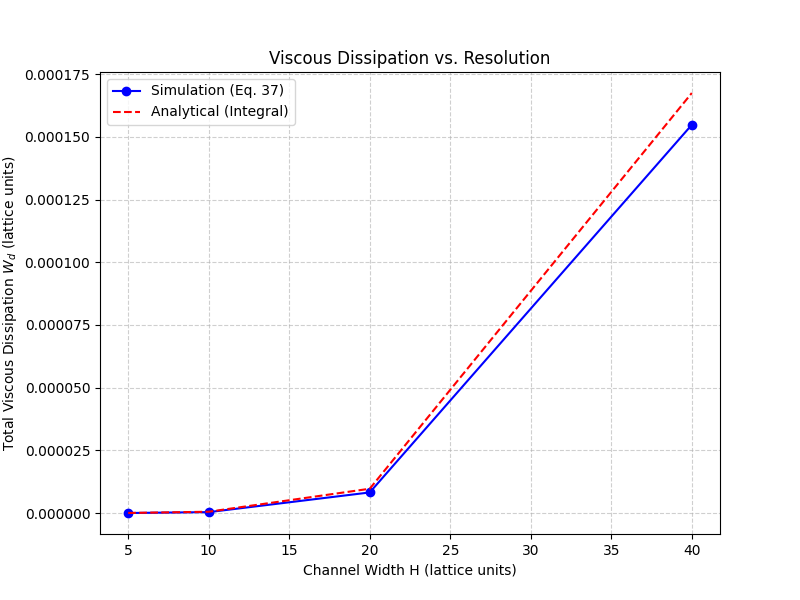
\includegraphics[width=0.7\textwidth]{figures/dissipation_vs_resolution.png}
    \caption{Comparison of simulated viscous dissipation (Eq. 37) with the analytical value vs. channel resolution H.}
    \label{fig:dissipation}
\end{figure}

Discussion: According to Figure \ref{fig:dissipation}, how well does the simulated dissipation match the analytical value? Analyze the convergence behavior from the relative error plot (Figure \ref{fig:dissipation_err}). Does the accuracy improve with increasing resolution $H$? This validates the simulation's ability to capture energy dissipation correctly.

\section{Conclusion}
Summarize the key findings. Was the velocity profile accurately reproduced? How did the different force calculation methods perform? Was TRT effective in reducing slip? Did the simulated dissipation match the theory and the work done by gravity?

\section*{References}
List any external resources consulted (textbook, papers, online resources, AI tools like ChatGPT, Gemini Code Assist, etc.). Refer to the assignment PDF for specific references (Krüger et al., Guo et al., Latt et al.).
\begin{itemize}
    \item Krüger, T., Kusumaatmaja, H., Kuzmin, A., Shardt, O., Silva, G., & Viggen, E. M. (2017). \textit{The Lattice Boltzmann Method: Principles and Practice}. Springer.
    \item Guo, Z., Zheng, C., & Shi, B. (2002). Discrete lattice effects on the forcing term in the lattice Boltzmann method. \textit{Physical Review E}, 65(4), 046308.
    % \item Latt, J., et al. (2021). Palabos: A parallel lattice Boltzmann solver. Computers & Mathematics with Applications, 81, 334-350.
    \item Assignment Two PDF: CL 469 - Lattice Boltzmann method for fluid flow (Date: 31-03-25)
    \item (Add any other resources used, e.g., specific websites, AI tools)
\end{itemize}

\appendix
\section{Source Code Snippets (Optional)}
Key parts of the implementation can be included here using the `listings` package.

Example: Collision step implementation
\begin{lstlisting}[caption={BGK Collision with Guo Forcing in Simulation::collideBGK}, label={lst:bgk_collision}]
// ... inside collideBGK loop ...
 equilibrium(rho_node, ux_node, uy_node, feq_node.data());

 for (int i = 0; i < LBM::Q; ++i) {
     size_t pop_idx = idx(x, y, i);
     double Fi = 0.0;
     calculateForceTermBGK(i, rho_node, ux_node, uy_node, Fi);

     // Eq. 26 (BGK collision + Guo force term)
     f_new[pop_idx] = f[pop_idx] * (1.0 - params.omega) + params.omega * feq_node[i] + Fi;
 }
// ...
\end{lstlisting}

Example: Momentum Exchange Force Calculation
\begin{lstlisting}[caption={Momentum Exchange Force Calculation in Simulation::calculateForcesMomentumExchange (Excerpt for Bottom Wall)}, label={lst:me_force}]
// ... inside calculateForcesMomentumExchange loop ...
 // Bottom wall (y=0): Consider fluid nodes at y=1
 for (int i = 0; i < LBM::Q; ++i) {
     int fluid_y = 1;
     if (LBM::cy[i] < 0) { // Directions from fluid (y=1) to wall (y=0) (i=4, 7, 8)
         size_t pop_idx = idx(x, fluid_y, i); // f*_i at node (x, 1)
         double f_star_i = f_new[pop_idx]; // Use post-collision f_new

         // Based on momentum transferred across the link per step
         F_bottom_x += LBM::cx[i] * f_star_i;
         F_bottom_y += LBM::cy[i] * f_star_i;
     }
 }
// ...
\end{lstlisting}

\end{document} 